
Due to the detailed planning and development of the GUI elements during the first deliverable the creation of the main operations GUI elements were able to be completed rather swiftly. However there was an initial lag caused by the lack of familiarity with JavaFX and scene builder. After a few hours of familiarization, a FXML closely resembling the prototyped design was created for the main order screen.

\begin{figure}[H]
	\centering
	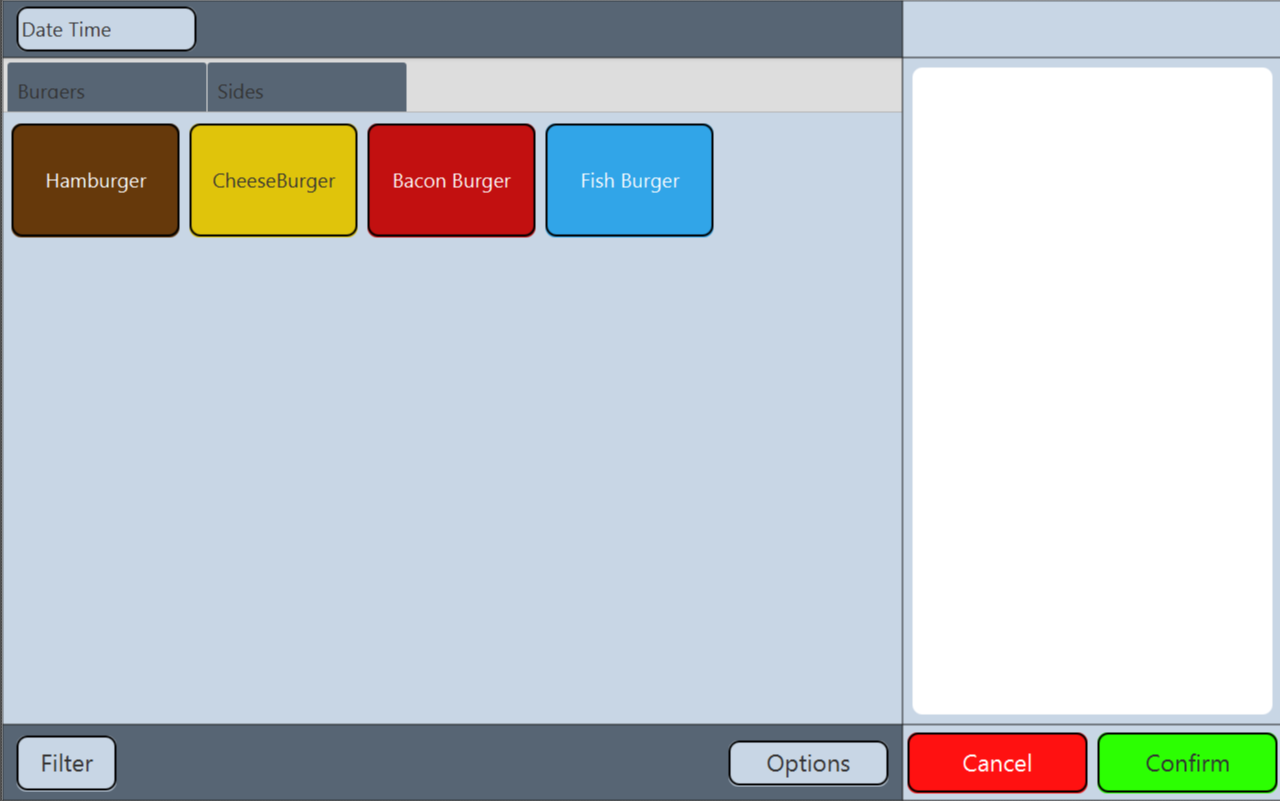
\includegraphics[width=150mm]{images/old_order_screen.png}
	\caption{Initial implementation of the prototyped design}
	\label{fig:old_order_screen}
\end{figure}

Most of the differences between the first implementation and the prototype (\ref{fig:old_order_screen} and \ref{fig:management_screen_moqueup} respectively) can be attributed to the differences between the programs used to create them as well as constraints created when implementing elements with relative alignments or elements that exist within other elements.

The first implementation of the GUI was effectively a simple skin of the prototype with buttons that printed their name but no further functionality. This allowed for development of basic skills and experience as well as a platform for further development moving forward. The experience gained from this base was then taken forward and used in creating other UI elements for the operations side whilst refining the main order screen and adding the functionality. The creation of these scenes and their functionality was significantly easier after getting over the initial learning curve of JavaFX and SceneBuilder.

During this time there was a conversation surrounding the implementation of the buttons for adding items to orders. Initially the buttons were designed and implemented to all be generated as blank, disabled buttons and then be enabled and filled when needed, however we decided to switch to an approach using buttons that were dynamically created and loaded when loading the main order screen in an effort to reduce cluttering of the main order window (QR3).

Through out the development of the operations side of the GUI small changes and adjustments were made to the design in an effort to clean and improve elements as they were noticed. An example of this was removing the black outline surrounding each item button. This change gave the main order screen a cleaner appearance, which was part of the driving force for the operational GUI.

The development of the management side GUI was unfortunately neglected during the planning stages so its development and implementation became plain and focused on the function when compared to the operations UIs. This caused the initial management screen prototype (see \ref{fig:management_screen_moqueup}) to be partially overhauled to a more tabular based approach that focused on presenting information and implementing functional elements in an efficient and simplified manner.

It is also worth noting that significant efforts towards planning and implementing the system architecture proved extremely valuable during the implementation of the functional elements and methods of the GUIs. This allowed for rapid implementation of features even when under time pressures close to the deliverable deadlines.

Retrospectively the development and implementation of the GUIs should be considered with a split between the operations and the management sides. This both reflects how the system functions as well as how the GUIs were implemented.

\pagebreak

\begin{figure}[h]
	\centering
	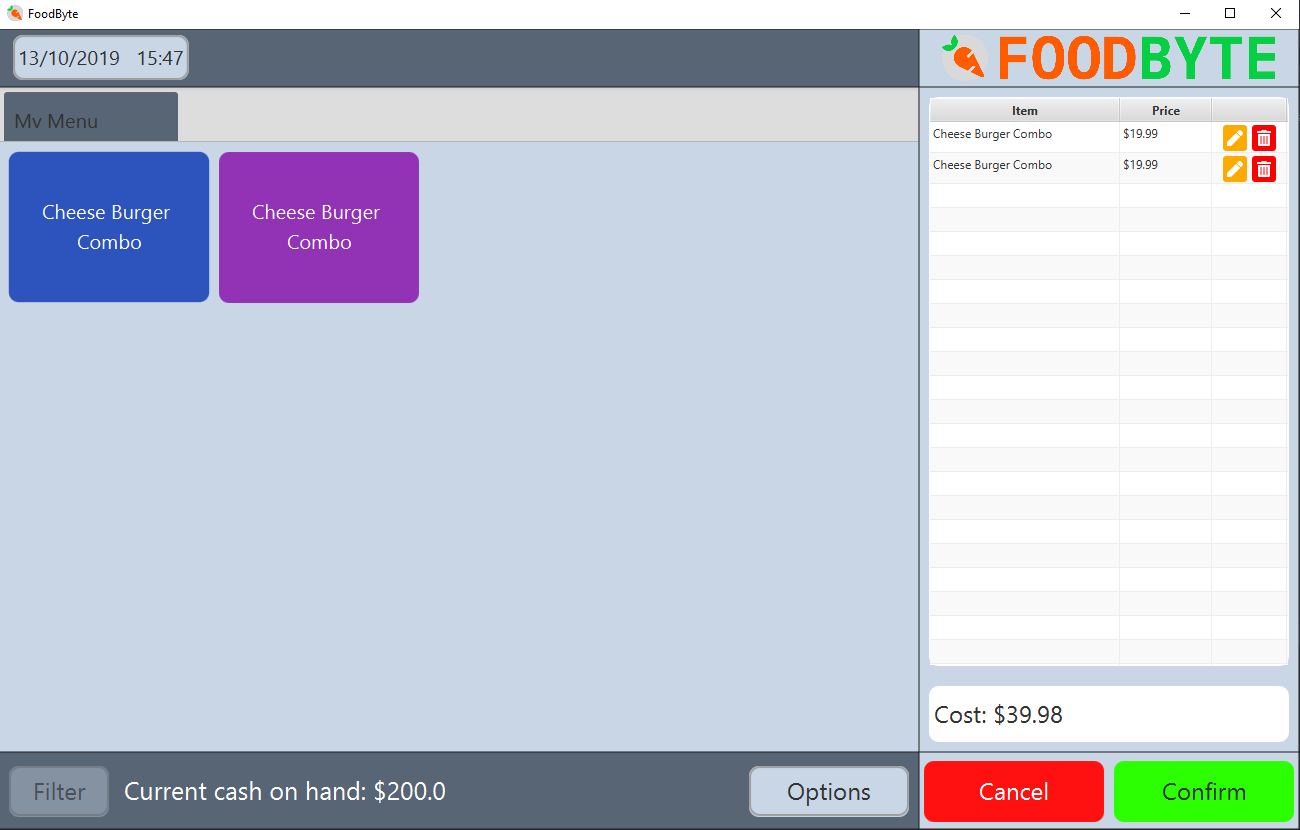
\includegraphics[width=150mm]{images/Final_GUI/main_order_screen.png}
	\caption{Final implementation of the main order screen}
	\label{fig:final_order_screen}
\end{figure}

The operations side was the major focus during both the planning and the implementation stages. Because of this there was a very clear plan and style that was carried through strongly into the implementation stages. This resulted in a final implementation (\ref{fig:final_order_screen}) that is very similar to the initial design with only a few minor aesthetics changes. The only major change between the prototype and the final implementation is the change from having pages with next/previous buttons to hold any overflow items for a given menu in the prototype, to a scrolling pane in the final implementation. This change was made, in spite of our earlier choice to the counter, because it allowed for easier scaling of the interface when the window size was changed whilst not making any major compromise towards usability.
\pagebreak

\begin{figure}[h]
	\centering
	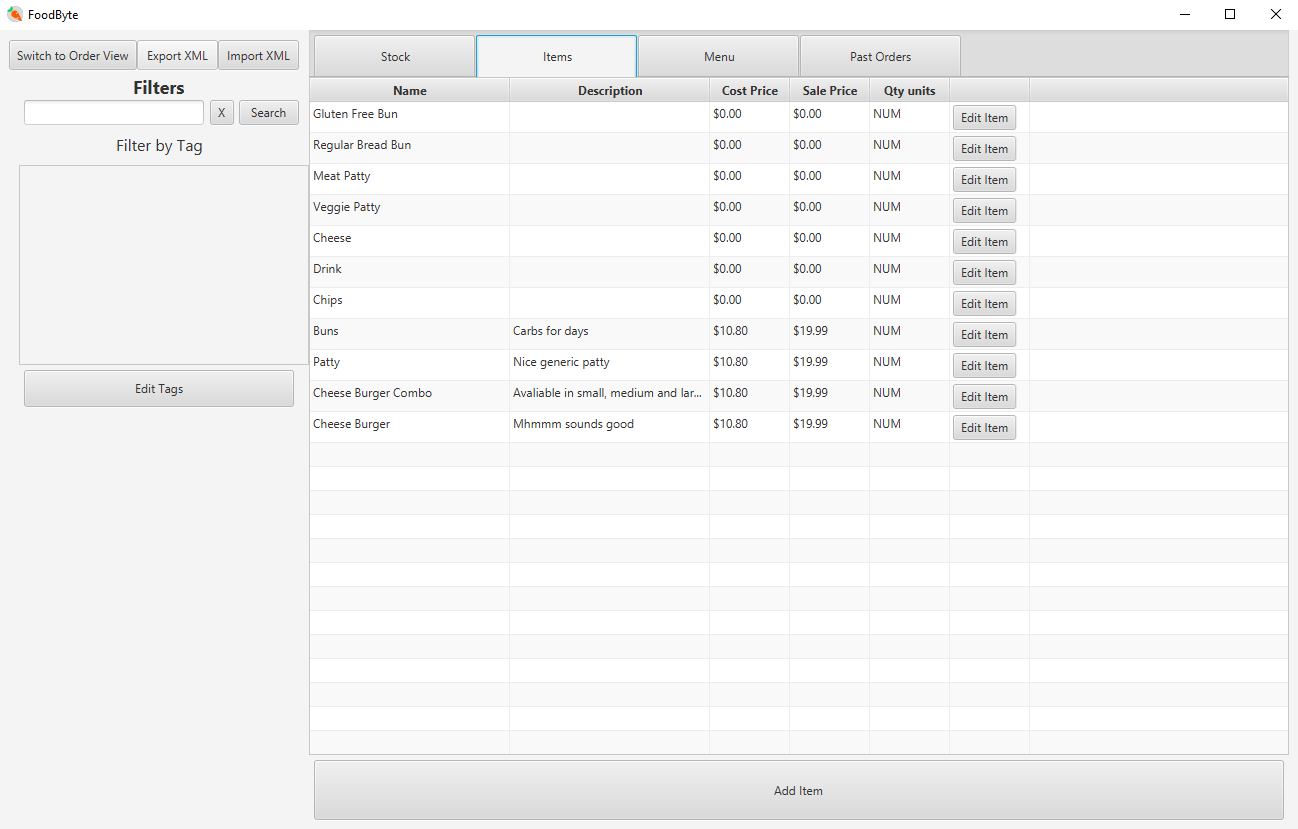
\includegraphics[width=150mm]{images/Final_GUI/item_screen.png}
	\caption{Final implementation of the item management screen}
	\label{fig:final_item_screen}
\end{figure}

The management side of the GUI was unfortunately neglected during the planning stage and this was also carried through to the implementation stage. During implementation the main focus was on creating function and although there was consideration and care towards usability there was little focus towards aesthetics. This has resulted in the management side not having the same visual standard as the operations side which is regrettable. The final management side UIs (example in \ref{fig:final_item_screen}) ended up implementing a stripped down tabular focused design. Although the management side is visually lacking when compared to the operations side it was agreed by the development team that, as the operations side will be the main focus of use during deployment, it was more important to have that to a high standard.

When retrospection the entire applications UIs as a whole it can be evidenced from the plans and the end result that heavier focus on the operations side has resulted in a application with a very clean and user friendly front end whilst and unfortunately lacklustre, in comparison, management side. If this project were to be further developed there is clear room to bring the management side up to the same stylized standard as the operations side and the style used in the operations side should be able to be ported into the management side without need for a complete redesign. It is also worth mentioning that there are areas in the options pop-up in the operations side that would allow for easy insertion of expanded features. On the management side this could also be accomplished by either adding more tabs to the tab pane or by pulling the tab pane down and using the row of space above that to implement more expansions.